En ésta segunda parte se especificará la naturaleza y las características de los campos que deben proveerse para alimentar y poder establecer una comunicación bidireccional entre el dispositivo de acoplamiento (\textit{PCD}) y las tarjetas de proximidad (\textit{PICC}). Como introducción sólo se presentará la interfaz de comunicación tipo A \cite{nfc_spec}.

\subsubsection{Términos y definiciones} 
\begin{itemize}
\item \textbf{Duración del bit:} Tiempo durante el cual un estado lógico es definido, al finalizar este un nuevo bit comienza.
\item \textbf{Modulación binaria por desplazamiento de fase:} Modulación de los estados con un desplazamiento de 180°, como resultado se tienen dos estados posibles.
\item \textbf{Índice de modulación:} Definido como $\frac{a-b}{a+b}$ donde a y b representan la máxima y mínima amplitud de la señal respectivamente.
\item \textbf{NRZ-L:} Método de codificación binaria mediante el cual un estado lógico posee la duración del bit y es representado por uno de dos estado físico definidos en el medio de comunicación.
\item \textbf{Subportadora:} La señal de RF producida por la modulación de una portadora de frecuencia fc con una señal de frecuencia fs.
\end{itemize}

\subsubsection{Diálogo inicial de las tarjetas de proximidad}

El diálogo inicial entre el PCD y el PICC debe respetar las siguientes operaciones en forma consecutiva.
Activar el PICC sometiéndolo al campo de RF generado por el PCD.
\begin{itemize}
\item El PICC entra al campo RF.
\item El PICC espera al comando del PCD.
\item El PCD transmite un comando.
\item El PICC transmite la respuesta.
\end{itemize}

Estas operaciones usan la energía de RF y la interfaz especificada en las siguientes cláusulas.

\begin{itemize}
\item \textbf{Transferencia de energía:} El PCD deberá producir un campo energizante de RF que acople el PICC para transferir la energía y el cual estará modulado para la comunicación.
\item \textbf{Frecuencia:} La frecuencia de la portadora (fc) deberá ser de 13.56MHz +- 7KHz.
\item \textbf{Campo operativo:} El campo mínimo sin modulación deberá ser de 1.5A/m (RMS) y el máximo de 7.5 A/m (RMS). Tanto el PCD como el PICC deberá operar entre estos rangos. El método para testear el campo generado por el PCD está definido en la ISO/IEC 10373.
\end{itemize}

\subsubsection{Interferencia de la señal}

Las dos interfaces de comunicación (tipo A y tipo B) están descriptas a continuación.

El PCD deberá alternar entre los métodos de modulación antes de la detección de la presencia de un PICC tipo A o tipo B. Sólo una interfaz de comunicación podrá estar activada durante una sesión de comunicación hasta la desactivación del PCD o la sustracción del PICC. La o las sesiones subsecuentes podrán proceder usando cualquier método de modulación. Los dos distintos tipos de interfaces se puede observar en la figura \ref{fig:tipos_iso}.

\begin{figure}[H]
\centering
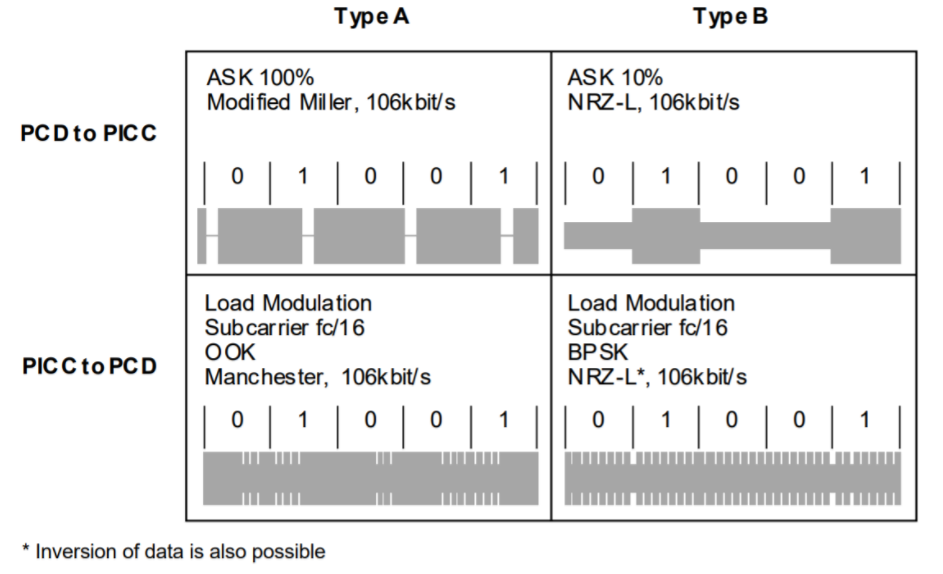
\includegraphics[width=0.9\linewidth]{otros/tipos_iso.png}
\caption{Tipos de inteface ISO/IEC 14443}
\label{fig:tipos_iso}
\end{figure}

\subsubsection{Interfaz de comunicación tipo “A”}

\begin{enumerate}
\item Comunicación PCD a PICC
\begin{itemize}
\item \textbf{Velocidad de transmisión:} durante la inicialización y anticolisión la velocidad de transmisión deberá ser fc/128.
\item \textbf{Modulación:} La comunicación entre el PCD y el PICC se lleva a cabo empleando el principio de modulación ASK 100\% del campo RF para crear la “pausa” como se muestra en la figura \ref{fig:demod_tipoa}.

\begin{figure}[H]
\centering
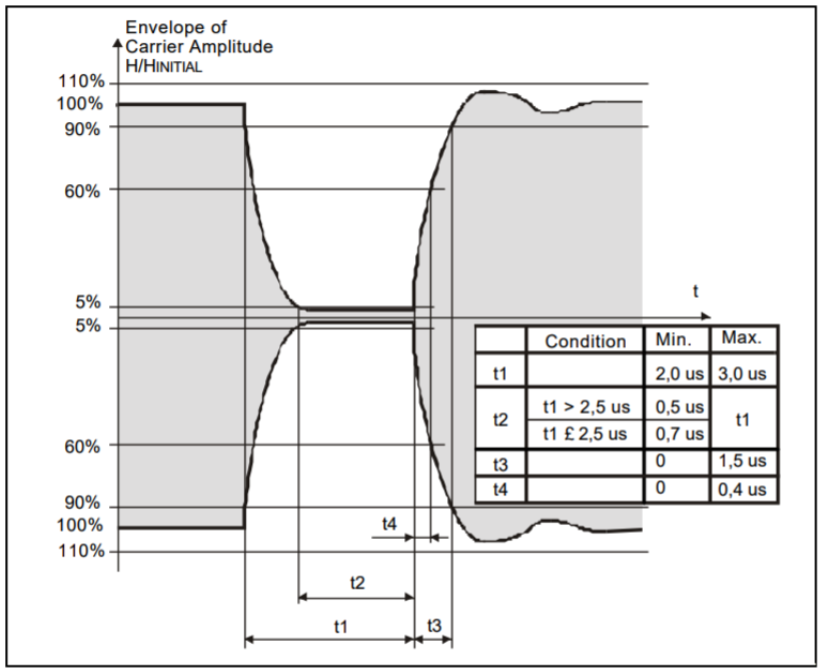
\includegraphics[width=0.7\linewidth]{otros/demod_tipoa.png}
\caption{Modulación PCD a PICC}
\label{fig:demod_tipoa}
\end{figure}

La envolvente del campo del PCD deberá decrementar monótonamente a menos del 5\% de su valor inicial (Hinicial) y permanecer de esta manera por un tiempo mayor a “t2”.

Si la envolvente del campo del PCD no decrementa monótonamente, el tiempo entre un máximo local y el tiempo del paso del mismo valor antes del máximo local no deberá exceder  los 0.5us. Esto solo aplicará si el máximo local es mayor al 5\% del H inicial.

El sobrepaso deberá permanecer entre el 90\% y el 110\% del H inicial.

El PICC deberá detectar el “Fin de pausa” (End of Pause) luego de que el campo exceda el 5\% del H inicial y antes de que supere el 60\% del mismo.

En la figura \ref{fig:pausa_tipoa} se procede a mostrar la definición del “Fin de Pausa” (EoP).

\begin{figure}[H]
\centering
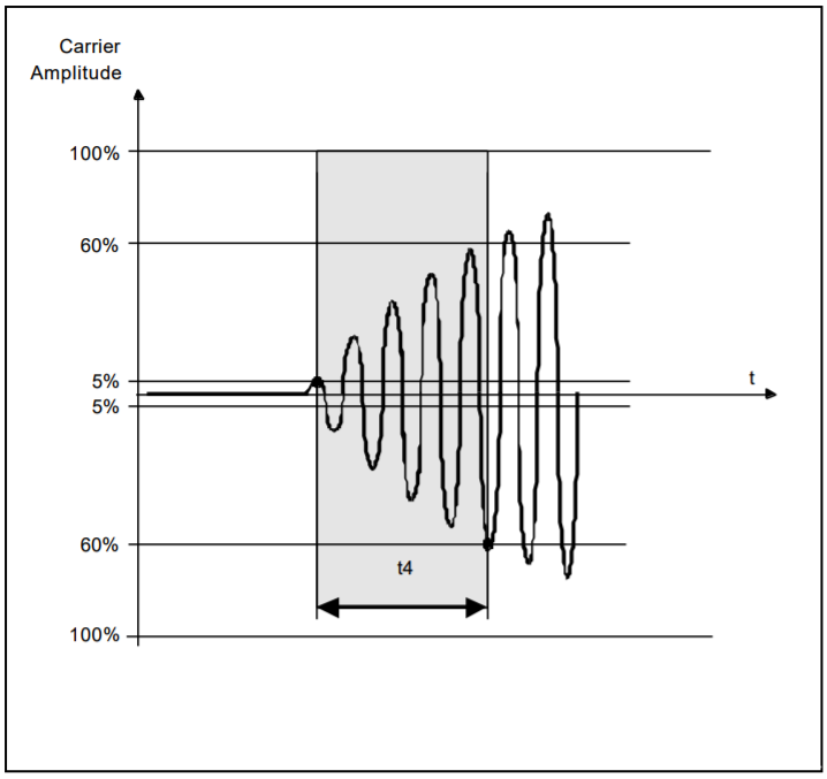
\includegraphics[width=0.7\linewidth]{otros/pausa_tipoa.png}
\caption{Fin de la pausa - ISO/IEC 14443A}
\label{fig:pausa_tipoa}
\end{figure}

\item \textbf{Representación de los bits y codificación:} Las secuencias están definidas en la tabla \ref{fig:code_tipoa} y la codificación en la tabla \ref{fig:dem_cod_tipoa}.

\begin{figure}[H]
\centering
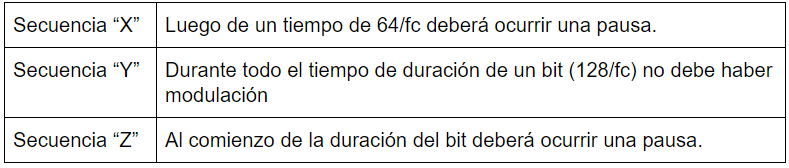
\includegraphics[width=0.9\linewidth]{otros/secuencia_tipoa.png}
\caption{Secuencia PCD a PICC}
\label{fig:code_tipoa}
\end{figure}

\begin{figure}[H]
\centering
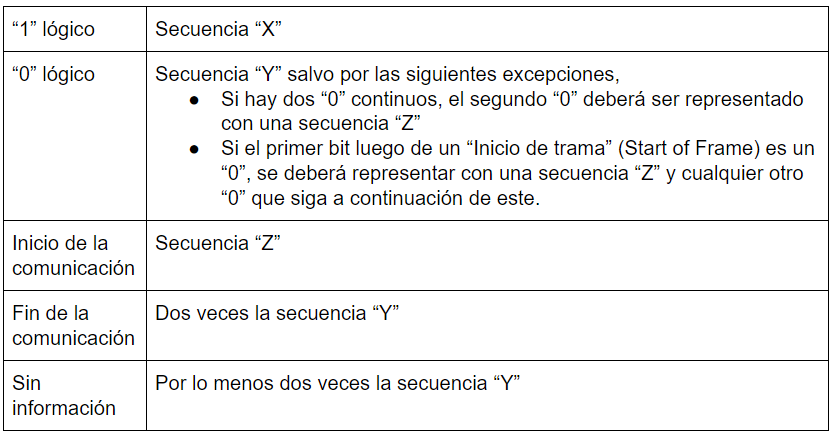
\includegraphics[width=0.9\linewidth]{otros/dem_codigo_tipoa.png}
\caption{Codificación PCD a PICC}
\label{fig:dem_cod_tipoa}
\end{figure}


\end{itemize}

\item Comunicación PICC a PCD

\begin{itemize}
\item \textbf{Velocidad de la información:} Al igual que la comunicación del PCD al PICC, la velocidad durante la inicialización y la anticolisión deberá ser de fc/128 (106 kbit/s).
\item \textbf{Carga de la modulación:} El PICC debera ser capaz de comunicarse hacía el PCD a través del acoplamiento inductivo en donde la frecuencia de la portadora será empleada para generar una subportadora de frecuencia fs. Esta subportadora deberá ser generada empleando una carga en el PICC. La amplitud de la modulación deberá ser por lo menos de 30/H mV, en donde H será el valor RMS de la fuerza del campo magnético en A/m.
\item \textbf{Subportadora:} La frecuencia fs debe ser de fc/16 (847kHz). Consecuentemente con esto, durante la inicialización y la anticolisión, la duración de un bit será equivalente a 8 periodos de la subportadora.
\item \textbf{Modulación de la subportadora:} Cada bit comienza su periodo con una fase definida en relación con la subportadora. El periodo del mismo comienza con el estado cargado de la subportadora. Esta deberá ser modulada usando modulacion on/off con las secuencias definidas en la tabla \ref{fig:mod_cod_tipoa}.

\begin{figure}[H]
\centering
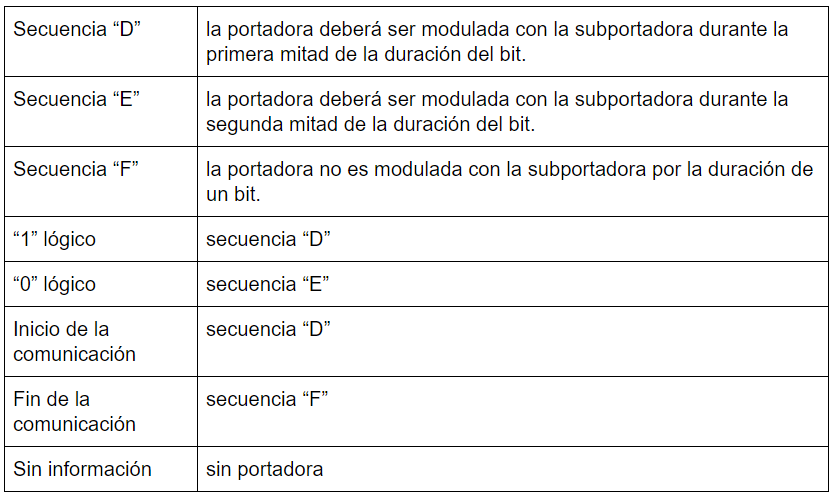
\includegraphics[width=0.9\linewidth]{otros/mod_codigo_tipoa.png}
\caption{Codificación PICC a PCD}
\label{fig:mod_cod_tipoa}
\end{figure}

\end{itemize}


\end{enumerate}